\documentclass[a4paper,12pt,twoside]{book}
\usepackage[utf8]{inputenc}
\usepackage[spanish,es-nodecimaldot,es-tabla]{babel}
\usepackage[left=2cm,right=2cm,top=2cm,bottom=3cm]{geometry}
\usepackage{graphicx}
\usepackage[notransparent]{svg} % Incluir imágenes en formato vectorial
\usepackage{minitoc} % Permite insertar índices de secciones dentro de cada capítulo
\usepackage[explicit]{titlesec} %para construir el formato de cada capitulo
\usepackage{type1cm}
\usepackage{amssymb}
\usepackage{stackengine}
\usepackage{pdfpages}
\usepackage{amsmath}
\usepackage{enumerate}
\usepackage{subcaption}
\usepackage{bm} % Fórmulas en negrita
\usepackage{algorithm}
\usepackage{algorithmic}
\usepackage{multirow}
\usepackage[figuresright]{rotating}
\usepackage[style=alphabetic, 
			isbn=false,     % whether the fields isbn/issn/isrn
			url=false,      % affects entry types whose url information is optional
			doi=false, backend=bibtex]{biblatex}
\usepackage{csquotes}
\usepackage{setspace}
\usepackage{tocloft} % Personalizar el indice
\usepackage{rotating} % Modificar orientación de figuras y tablas
\usepackage{booktabs}
\usepackage{afterpage,lscape} % Cambiar la orientación de una página
\usepackage{fancyhdr} % Configurar el contenido de las cabeceras
\usepackage{float}
\usepackage{enumitem} % Configurar separación entre items en listas numeradas
\setlist[itemize]{noitemsep} % Para eliminar la separación entre items
\setlist[enumerate]{noitemsep} % Para eliminar la separación entre items
\usepackage{microtype} % Bibliografia dentro de los márgenes
\usepackage{afterpage}
\usepackage{pdfpages}
\usepackage{titlesec}
\usepackage{epigraph}
\usepackage{datetime}
\usepackage{tikz} % Paquete para dibujar gráficos
\usepackage[export]{adjustbox}
\usetikzlibrary{datavisualization}
% Manejo de tablas
\usepackage{tabularx}
\usepackage{threeparttable}
\usepackage{makecell,booktabs}
\usepackage{amsthm}
\usepackage[hidelinks]{hyperref} % Ponerlo en este lugar para que las notas a pie de página funcionen.
\usepackage{xcolor} 
\usepackage{framed, color, verbatim}

% Paquetes extra %
%\usepackage{lettrine} % Poner letras de un tamaño mayor. Por ejemplo, para escribir la primera palabra de cada capítulo de tamaño mayor al resto
%\usepackage{kpfonts} % Tipo de letra. En concreto para que la primera letra de cada capitulo sea mas grande
%\usepackage[allfiguresdraft]{draftfigure} % Para no mostrar imágenes en tiempo de compilación.
%\usepackage{acronym}
% Numeración de capítulos con números romanos
%\renewcommand{\thechapter}{\Roman{chapter}}
%\setlist[itemize]{itemsep=0.5pt}

% Entorno verbatim para código MultiCalib4DEB
\definecolor{shadecolor}{rgb}{.9, .9, .9}

\newenvironment{code}%
{\snugshade\verbatim}%
{\endverbatim\endsnugshade}

% Acrónimos y pop-up asociados
\usepackage[only-used = true]{acro}
\usepackage{pdfcomment}
\acsetup{
	% make-links = true, 
	pdfcomments/use = true ,
}

% Definición del símbolo triángulo + igual
\def\delequal{\mathrel{\ensurestackMath{\stackon[1pt]{=}{\scriptstyle\Delta}}}}

\theoremstyle{remark}
\newtheorem*{remark}{Remark}

\newcommand\blankpage{%
    \null
    \thispagestyle{empty}%
    \addtocounter{page}{-1}%
    \newpage}

% Change point by colon between volumen and number of citation. 
\newcommand*{\volnumdelim}{\adddot}

\renewbibmacro*{volume+number+eid}{%
	\printfield{volume}%
	\setunit*{\addcolon}%
	\printfield{number}%
	\setunit{\addcomma\space}%
	\printfield{eid}}

\renewcommand*{\volnumdelim}{}

\addbibresource{bibliografia/biblio.bib}

\documentclass[a4paper,12pt,twoside]{book}
\usepackage[utf8]{inputenc}
\usepackage[spanish,es-nodecimaldot,es-tabla]{babel}
\usepackage[left=2cm,right=2cm,top=2cm,bottom=3cm]{geometry}
\usepackage{graphicx}
\usepackage[notransparent]{svg} % Incluir imágenes en formato vectorial
\usepackage{minitoc} % Permite insertar índices de secciones dentro de cada capítulo
\usepackage[explicit]{titlesec} %para construir el formato de cada capitulo
\usepackage{type1cm}
\usepackage{amssymb}
\usepackage{stackengine}
\usepackage{pdfpages}
\usepackage{amsmath}
\usepackage{enumerate}
\usepackage{subcaption}
\usepackage{bm} % Fórmulas en negrita
\usepackage{algorithm}
\usepackage{algorithmic}
\usepackage{multirow}
\usepackage[figuresright]{rotating}
\usepackage[style=alphabetic, 
			isbn=false,     % whether the fields isbn/issn/isrn
			url=false,      % affects entry types whose url information is optional
			doi=false, backend=bibtex]{biblatex}
\usepackage{csquotes}
\usepackage{setspace}
\usepackage{tocloft} % Personalizar el indice
\usepackage{rotating} % Modificar orientación de figuras y tablas
\usepackage{booktabs}
\usepackage{afterpage,lscape} % Cambiar la orientación de una página
\usepackage{fancyhdr} % Configurar el contenido de las cabeceras
\usepackage{float}
\usepackage{enumitem} % Configurar separación entre items en listas numeradas
\setlist[itemize]{noitemsep} % Para eliminar la separación entre items
\setlist[enumerate]{noitemsep} % Para eliminar la separación entre items
\usepackage{microtype} % Bibliografia dentro de los márgenes
\usepackage{afterpage}
\usepackage{pdfpages}
\usepackage{titlesec}
\usepackage{epigraph}
\usepackage{datetime}
\usepackage{tikz} % Paquete para dibujar gráficos
\usepackage[export]{adjustbox}
\usetikzlibrary{datavisualization}
% Manejo de tablas
\usepackage{tabularx}
\usepackage{threeparttable}
\usepackage{makecell,booktabs}
\usepackage{amsthm}
\usepackage[hidelinks]{hyperref} % Ponerlo en este lugar para que las notas a pie de página funcionen.
\usepackage{xcolor} 
\usepackage{framed, color, verbatim}

% Paquetes extra %
%\usepackage{lettrine} % Poner letras de un tamaño mayor. Por ejemplo, para escribir la primera palabra de cada capítulo de tamaño mayor al resto
%\usepackage{kpfonts} % Tipo de letra. En concreto para que la primera letra de cada capitulo sea mas grande
%\usepackage[allfiguresdraft]{draftfigure} % Para no mostrar imágenes en tiempo de compilación.
%\usepackage{acronym}
% Numeración de capítulos con números romanos
%\renewcommand{\thechapter}{\Roman{chapter}}
%\setlist[itemize]{itemsep=0.5pt}

% Entorno verbatim para código MultiCalib4DEB
\definecolor{shadecolor}{rgb}{.9, .9, .9}

\newenvironment{code}%
{\snugshade\verbatim}%
{\endverbatim\endsnugshade}

% Acrónimos y pop-up asociados
\usepackage[only-used = true]{acro}
\usepackage{pdfcomment}
\acsetup{
	% make-links = true, 
	pdfcomments/use = true ,
}

% Definición del símbolo triángulo + igual
\def\delequal{\mathrel{\ensurestackMath{\stackon[1pt]{=}{\scriptstyle\Delta}}}}

\theoremstyle{remark}
\newtheorem*{remark}{Remark}

\newcommand\blankpage{%
    \null
    \thispagestyle{empty}%
    \addtocounter{page}{-1}%
    \newpage}

% Change point by colon between volumen and number of citation. 
\newcommand*{\volnumdelim}{\adddot}

\renewbibmacro*{volume+number+eid}{%
	\printfield{volume}%
	\setunit*{\addcolon}%
	\printfield{number}%
	\setunit{\addcomma\space}%
	\printfield{eid}}

\renewcommand*{\volnumdelim}{}

\addbibresource{bibliografia/biblio.bib}

\documentclass[a4paper,12pt,twoside]{book}
\usepackage[utf8]{inputenc}
\usepackage[spanish,es-nodecimaldot,es-tabla]{babel}
\usepackage[left=2cm,right=2cm,top=2cm,bottom=3cm]{geometry}
\usepackage{graphicx}
\usepackage[notransparent]{svg} % Incluir imágenes en formato vectorial
\usepackage{minitoc} % Permite insertar índices de secciones dentro de cada capítulo
\usepackage[explicit]{titlesec} %para construir el formato de cada capitulo
\usepackage{type1cm}
\usepackage{amssymb}
\usepackage{stackengine}
\usepackage{pdfpages}
\usepackage{amsmath}
\usepackage{enumerate}
\usepackage{subcaption}
\usepackage{bm} % Fórmulas en negrita
\usepackage{algorithm}
\usepackage{algorithmic}
\usepackage{multirow}
\usepackage[figuresright]{rotating}
\usepackage[style=alphabetic, 
			isbn=false,     % whether the fields isbn/issn/isrn
			url=false,      % affects entry types whose url information is optional
			doi=false, backend=bibtex]{biblatex}
\usepackage{csquotes}
\usepackage{setspace}
\usepackage{tocloft} % Personalizar el indice
\usepackage{rotating} % Modificar orientación de figuras y tablas
\usepackage{booktabs}
\usepackage{afterpage,lscape} % Cambiar la orientación de una página
\usepackage{fancyhdr} % Configurar el contenido de las cabeceras
\usepackage{float}
\usepackage{enumitem} % Configurar separación entre items en listas numeradas
\setlist[itemize]{noitemsep} % Para eliminar la separación entre items
\setlist[enumerate]{noitemsep} % Para eliminar la separación entre items
\usepackage{microtype} % Bibliografia dentro de los márgenes
\usepackage{afterpage}
\usepackage{pdfpages}
\usepackage{titlesec}
\usepackage{epigraph}
\usepackage{datetime}
\usepackage{tikz} % Paquete para dibujar gráficos
\usepackage[export]{adjustbox}
\usetikzlibrary{datavisualization}
% Manejo de tablas
\usepackage{tabularx}
\usepackage{threeparttable}
\usepackage{makecell,booktabs}
\usepackage{amsthm}
\usepackage[hidelinks]{hyperref} % Ponerlo en este lugar para que las notas a pie de página funcionen.
\usepackage{xcolor} 
\usepackage{framed, color, verbatim}

% Paquetes extra %
%\usepackage{lettrine} % Poner letras de un tamaño mayor. Por ejemplo, para escribir la primera palabra de cada capítulo de tamaño mayor al resto
%\usepackage{kpfonts} % Tipo de letra. En concreto para que la primera letra de cada capitulo sea mas grande
%\usepackage[allfiguresdraft]{draftfigure} % Para no mostrar imágenes en tiempo de compilación.
%\usepackage{acronym}
% Numeración de capítulos con números romanos
%\renewcommand{\thechapter}{\Roman{chapter}}
%\setlist[itemize]{itemsep=0.5pt}

% Entorno verbatim para código MultiCalib4DEB
\definecolor{shadecolor}{rgb}{.9, .9, .9}

\newenvironment{code}%
{\snugshade\verbatim}%
{\endverbatim\endsnugshade}

% Acrónimos y pop-up asociados
\usepackage[only-used = true]{acro}
\usepackage{pdfcomment}
\acsetup{
	% make-links = true, 
	pdfcomments/use = true ,
}

% Definición del símbolo triángulo + igual
\def\delequal{\mathrel{\ensurestackMath{\stackon[1pt]{=}{\scriptstyle\Delta}}}}

\theoremstyle{remark}
\newtheorem*{remark}{Remark}

\newcommand\blankpage{%
    \null
    \thispagestyle{empty}%
    \addtocounter{page}{-1}%
    \newpage}

% Change point by colon between volumen and number of citation. 
\newcommand*{\volnumdelim}{\adddot}

\renewbibmacro*{volume+number+eid}{%
	\printfield{volume}%
	\setunit*{\addcolon}%
	\printfield{number}%
	\setunit{\addcomma\space}%
	\printfield{eid}}

\renewcommand*{\volnumdelim}{}

\addbibresource{bibliografia/biblio.bib}

\documentclass[a4paper,12pt,twoside]{book}
\usepackage[utf8]{inputenc}
\usepackage[spanish,es-nodecimaldot,es-tabla]{babel}
\usepackage[left=2cm,right=2cm,top=2cm,bottom=3cm]{geometry}
\usepackage{graphicx}
\usepackage[notransparent]{svg} % Incluir imágenes en formato vectorial
\usepackage{minitoc} % Permite insertar índices de secciones dentro de cada capítulo
\usepackage[explicit]{titlesec} %para construir el formato de cada capitulo
\usepackage{type1cm}
\usepackage{amssymb}
\usepackage{stackengine}
\usepackage{pdfpages}
\usepackage{amsmath}
\usepackage{enumerate}
\usepackage{subcaption}
\usepackage{bm} % Fórmulas en negrita
\usepackage{algorithm}
\usepackage{algorithmic}
\usepackage{multirow}
\usepackage[figuresright]{rotating}
\usepackage[style=alphabetic, 
			isbn=false,     % whether the fields isbn/issn/isrn
			url=false,      % affects entry types whose url information is optional
			doi=false, backend=bibtex]{biblatex}
\usepackage{csquotes}
\usepackage{setspace}
\usepackage{tocloft} % Personalizar el indice
\usepackage{rotating} % Modificar orientación de figuras y tablas
\usepackage{booktabs}
\usepackage{afterpage,lscape} % Cambiar la orientación de una página
\usepackage{fancyhdr} % Configurar el contenido de las cabeceras
\usepackage{float}
\usepackage{enumitem} % Configurar separación entre items en listas numeradas
\setlist[itemize]{noitemsep} % Para eliminar la separación entre items
\setlist[enumerate]{noitemsep} % Para eliminar la separación entre items
\usepackage{microtype} % Bibliografia dentro de los márgenes
\usepackage{afterpage}
\usepackage{pdfpages}
\usepackage{titlesec}
\usepackage{epigraph}
\usepackage{datetime}
\usepackage{tikz} % Paquete para dibujar gráficos
\usepackage[export]{adjustbox}
\usetikzlibrary{datavisualization}
% Manejo de tablas
\usepackage{tabularx}
\usepackage{threeparttable}
\usepackage{makecell,booktabs}
\usepackage{amsthm}
\usepackage[hidelinks]{hyperref} % Ponerlo en este lugar para que las notas a pie de página funcionen.
\usepackage{xcolor} 
\usepackage{framed, color, verbatim}

% Paquetes extra %
%\usepackage{lettrine} % Poner letras de un tamaño mayor. Por ejemplo, para escribir la primera palabra de cada capítulo de tamaño mayor al resto
%\usepackage{kpfonts} % Tipo de letra. En concreto para que la primera letra de cada capitulo sea mas grande
%\usepackage[allfiguresdraft]{draftfigure} % Para no mostrar imágenes en tiempo de compilación.
%\usepackage{acronym}
% Numeración de capítulos con números romanos
%\renewcommand{\thechapter}{\Roman{chapter}}
%\setlist[itemize]{itemsep=0.5pt}

% Entorno verbatim para código MultiCalib4DEB
\definecolor{shadecolor}{rgb}{.9, .9, .9}

\newenvironment{code}%
{\snugshade\verbatim}%
{\endverbatim\endsnugshade}

% Acrónimos y pop-up asociados
\usepackage[only-used = true]{acro}
\usepackage{pdfcomment}
\acsetup{
	% make-links = true, 
	pdfcomments/use = true ,
}

% Definición del símbolo triángulo + igual
\def\delequal{\mathrel{\ensurestackMath{\stackon[1pt]{=}{\scriptstyle\Delta}}}}

\theoremstyle{remark}
\newtheorem*{remark}{Remark}

\newcommand\blankpage{%
    \null
    \thispagestyle{empty}%
    \addtocounter{page}{-1}%
    \newpage}

% Change point by colon between volumen and number of citation. 
\newcommand*{\volnumdelim}{\adddot}

\renewbibmacro*{volume+number+eid}{%
	\printfield{volume}%
	\setunit*{\addcolon}%
	\printfield{number}%
	\setunit{\addcomma\space}%
	\printfield{eid}}

\renewcommand*{\volnumdelim}{}

\addbibresource{bibliografia/biblio.bib}

\include{thesis.preamble}

%%%%%%%%%%%%%%%%%%%%%%%%%%%%%
%% ACRÓNIMOS
%%%%%%%%%%%%%%%%%%%%%%%%%%%%%
% Acrónimos Inglés
\DeclareAcronym{AO}{
	short = AI ,
	short-plural = es,
	long = {Acronym One},
	long-plural = es ,
	pdfcomment = {Acronym One}
}
%%%%%%%%%%%%%%%%%%%%%%%%%%
%%% FIN ACRÓNIMOS
%%%%%%%%%%%%%%%%%%%%%%%%%%

\begin{document}

\title{\hrule\LARGE {\bf Título Tesis\vspace*{2mm}\hrule}\par
 \vspace*{6mm}
}

\author{\textbf{Nombre y Apellidos Doctorando}}

\normallinespacing

\maketitle

%\preface % Eliminado porque añade dos páginas blancas tras primera entrada del documento. 
\newpage
\thispagestyle{empty}
\mbox{}
\newpage
\input{citas/citas}
\newpage
\thispagestyle{empty}
\mbox{}
\newpage
\input{agradecimientos/agradecimientos}
\newpage
\thispagestyle{empty}
\mbox{}
\newpage
\input{declaraciones/supervision}
\newpage
\thispagestyle{empty}
\mbox{}
\newpage
\input{glosario/acronimos}
\newpage
\thispagestyle{empty}

% Numeración de páginas con números romanos previa a los capítulos.
\singlespacing
\pagenumbering{Roman}
\setcounter{page}{11}
\body

\chapter*{Resumen}\label{capitulo:Resumen}
\markboth{Resumen}{}
\input{resumen/resumen}
\addcontentsline{toc}{chapter}{Resumen}
\clearpage
\chapter*{Abstract}\label{capitulo:Abstract}
\markboth{}{}
\input{abstract/abstract}
\addcontentsline{toc}{chapter}{Abstract}
\clearpage
\chapter{Introducción}\label{capitulo:Introduccion}
\input{introduccion/introduccion}
\clearpage
\part{Fundamentos}
\clearpage
\chapter{Capítulo dos}\label{capitulo:CapituloDos}
\input{capitulos/Fundamentos/CapituloDos}
\chapter{Capítulo tres}\label{capitulo:CapituloTres}
\input{capitulos/Fundamentos/CapituloTres}
\clearpage
\part{Propuesta}
\clearpage
\chapter{Capítulo cuatro}\label{capitulo:CapituloCuatro}
\input{capitulos/Propuesta/CapituloCuatro}
\clearpage
\part{Observaciones finales}
\clearpage
\chapter{Conclusiones y trabajos futuros}\label{capitulo:Conclusiones}
\input{conclusiones/conclusiones}
\clearpage

\addcontentsline{toc}{chapter}{Bibliografía}
\printbibliography

\end{document}

%%%%%%%%%%%%%%%%%%%%%%%%%%%%%
%% ACRÓNIMOS
%%%%%%%%%%%%%%%%%%%%%%%%%%%%%
% Acrónimos Inglés
\DeclareAcronym{AO}{
	short = AI ,
	short-plural = es,
	long = {Acronym One},
	long-plural = es ,
	pdfcomment = {Acronym One}
}
%%%%%%%%%%%%%%%%%%%%%%%%%%
%%% FIN ACRÓNIMOS
%%%%%%%%%%%%%%%%%%%%%%%%%%

\begin{document}

\title{\hrule\LARGE {\bf Título Tesis\vspace*{2mm}\hrule}\par
 \vspace*{6mm}
}

\author{\textbf{Nombre y Apellidos Doctorando}}

\normallinespacing

\maketitle

%\preface % Eliminado porque añade dos páginas blancas tras primera entrada del documento. 
\newpage
\thispagestyle{empty}
\mbox{}
\newpage
\narrowlinespacing

\vspace*{5cm}

\epigraph{Primera cita.}{Autor}

\normallinespacing
\newpage
\thispagestyle{empty}
\mbox{}
\newpage

\begin{acknowledgements}

Agradecimientos de la tesis. La parte más importante de la tesis.

\begin{center}
Mensaje centrado.
\end{center}

\end{acknowledgements}
\newpage
\thispagestyle{empty}
\mbox{}
\newpage
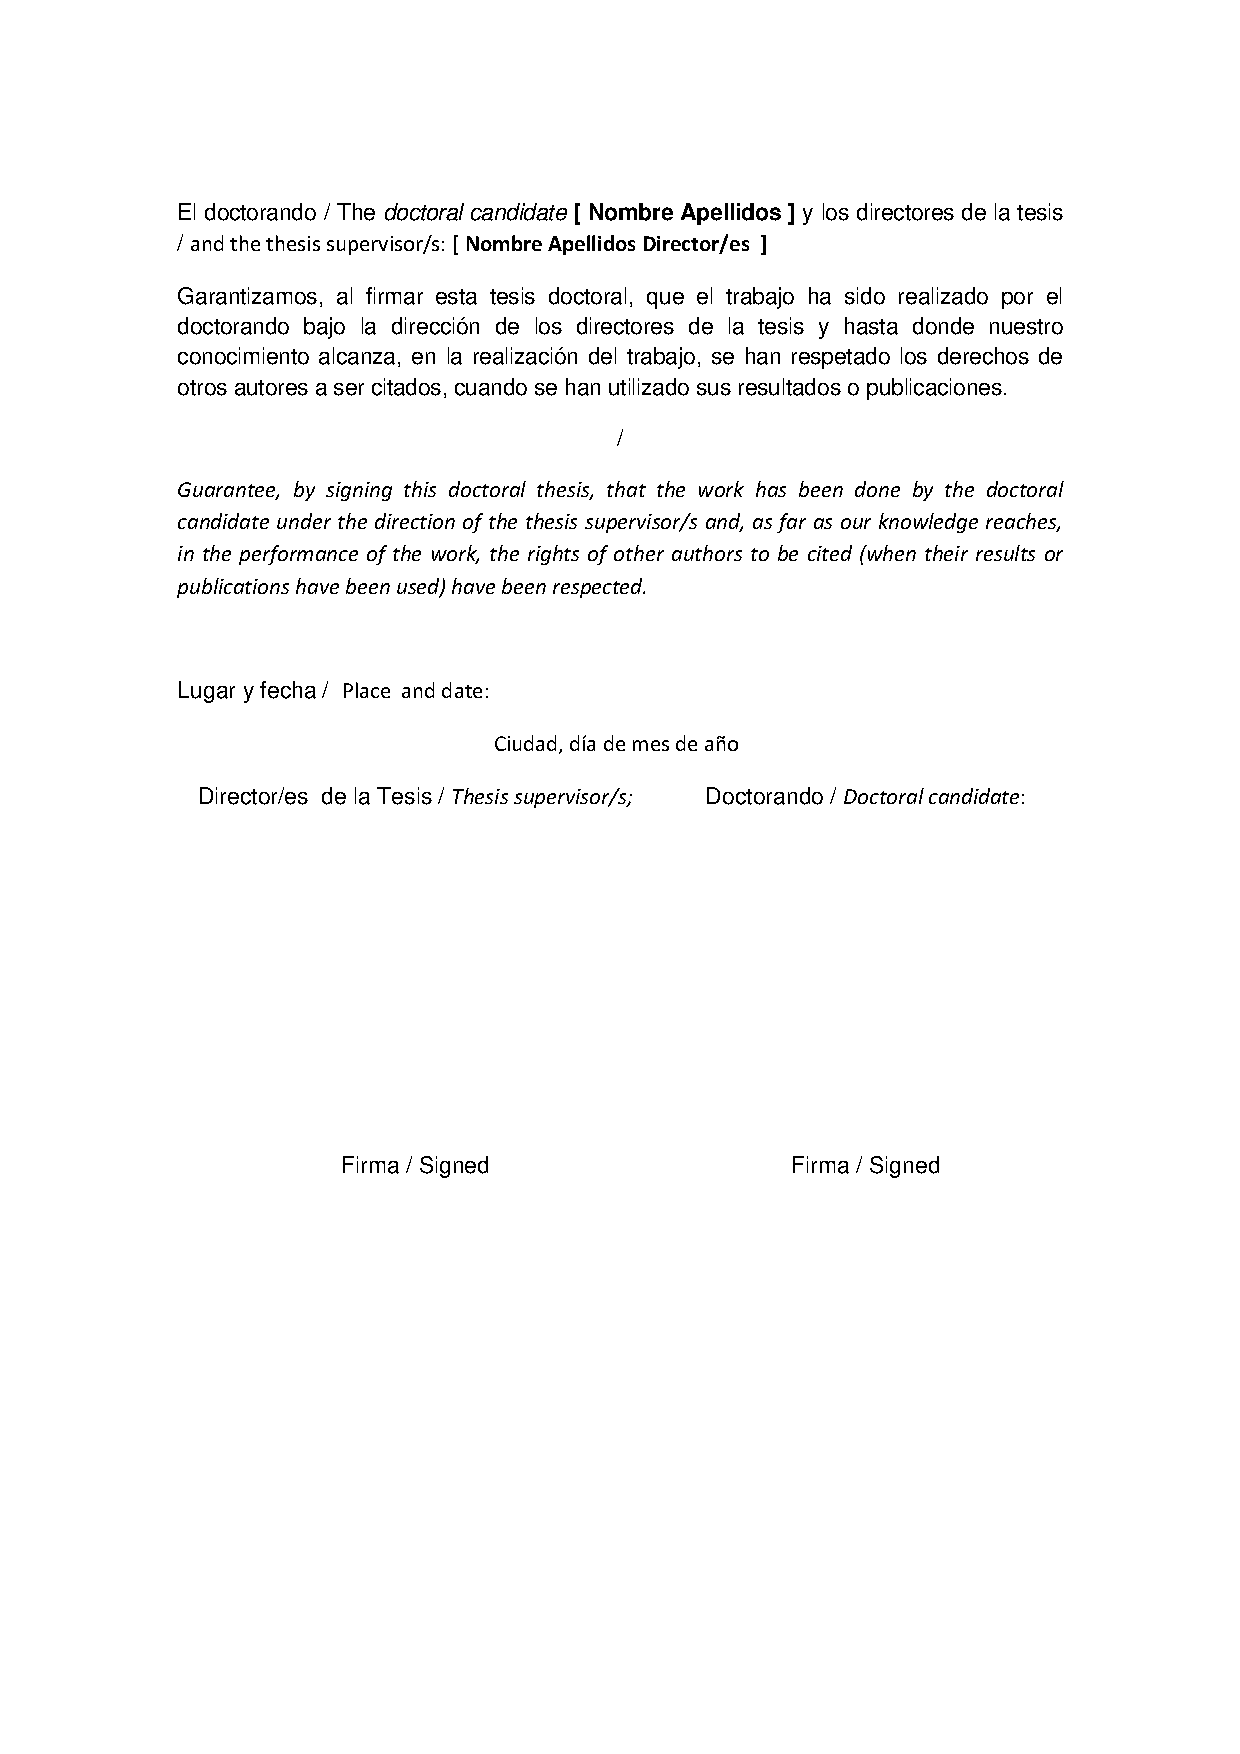
\includepdf[offset=15 0]{declaraciones/Compromiso_derechos_autor_tesis_firmado.pdf}
\newpage
\thispagestyle{empty}
\mbox{}
\newpage
{\large\bf Acrónimos}
\printacronyms[heading=none]
\newpage
\thispagestyle{empty}

% Numeración de páginas con números romanos previa a los capítulos.
\singlespacing
\pagenumbering{Roman}
\setcounter{page}{11}
\body

\chapter*{Resumen}\label{capitulo:Resumen}
\markboth{Resumen}{}

%\mtcaddchapter[Resumen] %Para añadirlo al indice y que no genere conflicto con el paquete minitoc

\section*{Introducción al problema}\label{seccion:IntroduccionProblema}

Introducción al problema abordado.

\section*{Desarrollo}\label{seccion:Desarrollo}

Bloques desarrollo de tesis: 

\begin{enumerate}[label=\Roman*]
	\item Bloque A.
	\item Bloque B. 
	\item Bloque C.
\end{enumerate}

Introducción a secciones tesis. 

\subsection*{Sección uno}\label{seccion:SeccionUno}

Iniciamos \dots 

\subsection*{Sección dos}\label{seccion:SeccionDos}

Tras finalizar la Sección~\ref{seccion:SeccionUno} \dots

\subsection*{Sección tres}\label{seccion:SeccionTres}

Como ya mencionamos en \dots 

\subsection*{Sección cuatro}\label{seccion:SeccionCuatro}

Por último \dots

\section*{Conclusiones y trabajos futuros}\label{seccion:ConclusionesResumen}

En conclusión \dots


\addcontentsline{toc}{chapter}{Resumen}
\clearpage
\chapter*{Abstract}\label{capitulo:Abstract}
\markboth{}{}
%\newpage
%\thispagestyle{empty}
%\mbox{}
%\newpage

%\mtcaddchapter[Resumen] %Para añadirlo al indice y que no genere conflicto con el paquete minitoc

%\begin{resumen}
%\input{resumen/resumen}
%\end{resumen}
    
%\newpage
%\thispagestyle{empty}
%\mbox{}
%\newpage

%\mtcaddchapter[Abstract]

Abstract written in English \dots
\addcontentsline{toc}{chapter}{Abstract}
\clearpage
\chapter{Introducción}\label{capitulo:Introduccion}

\epigraph{Cita.}{Autor}

\section{Introducción}\label{seccion:Introduccion}

\section{Objetivos}\label{seccion:Objetivos}

En esta tesis hemos de cumplir los siguientes objetivos específicos:

\begin{itemize}
	\item En nuestro \textbf{primer objetivo} \dots
	\item Un \textbf{segundo objetivo} \dots
    \item Un \textbf{tercer objetivo} \dots
\end{itemize}

\section{Estructura}\label{seccion:Estructura}

Esta tesis doctoral se divide en tres partes: Fundamentos, Propuesta y Observaciones finales, además de la presente introducción. 

La primera parte introduce al lector en los fundamentos de varias teorías y metodologías \dots En el capítulo~\ref{capitulo:CapituloUno} se \dots A continuación, en el capítulo~\ref{capitulo:CapituloDos}, se \dots

La segunda parte (Propuesta) desarrolla \dots Por un lado, el capítulo~\ref{capitulo:CapituloTres} describe \dots

Por último, la tercera parte (Observaciones finales), consta de un único capítulo (capítulo~\ref{capitulo:Conclusiones}) en el que \dots
\clearpage
\part{Fundamentos}
\clearpage
\chapter{Capítulo dos}\label{capitulo:CapituloDos}
\epigraph{Cita}{Autor}

\section{Sección uno}\label{seccion:SeccionUnoCapituloUno}

Las sociedades~\cite{citaEjemplo23} \dots
	
\section{Sección dos}\label{seccion:SeccionDosCapituloUno}

Una de \dots

\begin{itemize}
	\item \textbf{Uno}: Los \dots
	\item \textbf{Dos}: Los \dots
	\item \textbf{Tres}: Los \dots
	\item \textbf{Cuatro}: Los \dots
	\item \textbf{Cinco}: Los \dots
\end{itemize}

\section{Sección tres}\label{seccion:SeccionTresCapituloUno}

El acrónimo uno (\acsp{AO}, por sus siglas en inglés) \dots

\subsection{Subsección uno}\label{subsection:SubseccionUnoSeccionTresCapituloUno} 

\subsection{Subsección dos}\label{subseccion:SubseccionDosSeccionTresCapituloUno}

Las \dots

La Figura~\ref{figura:EjemploUno}
\begin{figure}[!ht]
	\centering
	\includesvg[width=7cm]{imagenes/logoUGR.svg}
	\caption{Figura de ejemplo}
	\label{figura:EjemploUno}
\end{figure}

\iffalse % Para guardar texto redactado como comentario para su posterior reutilización
\begin{itemize}
	\item \textbf{Ejemplo uno}:  
	\item \textbf{Ejemplo dos}: 
	\item \textbf{Ejemplo tres}: 
\end{itemize}
\fi

\subsubsection{Subsubsección uno}\label{subsubseccion:SubsubseccionUnoSubseccionUnoSeccionTresCapituloUno}

\subsubsection{Subsubsección dos}\label{subsubseccion:SubsubseccionDosSubseccionUnoSeccionTresCapituloUno}

\subsubsection{Subsubsección tres}\label{subsubseccion:SubsubseccionTresSubseccionUnoSeccionTresCapituloUno}

\subsection{Subsección tres}\label{subseccion:SubseccionTresSeccionTresCapituloUno} 

\subsubsection{Subsubsección uno}\label{subsubseccion:SubsubseccionUnoSubseccionTresSeccionTresCapituloUno}
\chapter{Capítulo tres}\label{capitulo:CapituloTres}
\epigraph{Cita.}{Autor}

\section{Sección uno}\label{seccion:SeccionUnoCapituloDos}

Como vimos en la Sección~\ref{seccion:SeccionUnoCapituloUno}, la tesis \dots

\section{Sección dos}\label{seccion:SeccionDosCapituloDos}
\clearpage
\part{Propuesta}
\clearpage
\chapter{Capítulo cuatro}\label{capitulo:CapituloCuatro}

\epigraph{Cita.}{Autor}

\section{Sección uno}\label{seccion:SeccionUnoCapituloTres}

En el Capítulo~\ref{capitulo:CapituloTres} expusimos \dots 

En la Table~\ref{tabla:EjemploUno} \dots

\begin{table}[H]
	\centering
	\footnotesize
	\begin{tabular}{|c||l||l|}
		\hline
		\textbf{Columna uno} & \textbf{Columna dos} & \textbf{Columna tres} \\ \hline \hline
		$A$ & I & 1\\ \hline
		$B$ & II & 2\\ \hline
		$C$ & III & 3\\ \hline
		$D$ & IV & 4\\ \hline
		$E$ & V & 5 \\ \hline
		\multirow{2}{*}{$F$} & \multirow{2}{*}{VI} & \multirow{2}{*}{\begin{tabular}[c]{@{}l@{}} $6, 7, 8, 9,$ \\  $10, 11, 12, 13$ \end{tabular}} \\ 
		& & \\ \hline
		\multirow{2}{*}{$G$} & \multirow{2}{*}{VII} & \multirow{2}{*}{\begin{tabular}[c]{@{}l@{}} $8, 9, 10, 11,$ \\ $10, 9, 8, 7$ \end{tabular}} \\
		& & \\
		\bottomrule
	\end{tabular}
	\caption{Tabla de ejemplo.}
	\label{tabla:EjemploUno}
\end{table}
\clearpage
\part{Observaciones finales}
\clearpage
\chapter{Conclusiones y trabajos futuros}\label{capitulo:Conclusiones}
\epigraph{Los hombres geniales empiezan grandes obras, los hombres trabajadores las terminan.}{Leonardo da Vinci}

\section{Conclusiones}\label{seccion:Conclusiones}

Las principales conclusiones de esta tesis son \dots 

\section{Publicaciones}\label{seccion:Publicaciones}

Por último, esta sección presenta las publicaciones científicas realizadas en el curso de esta tesis doctoral.

\textbf{Artículos publicados en revistas indexadas en el JCR-SCI (X):}

\begin{enumerate}
    \item Surname author I, Name author I, Surname author II, \& Name author II, O. (Year). \textbf{Paper Title}. Journal, Number, Pages. DOI: doi-number (JCR Year; impact: factor; Cat.: CATEGORY; Pos.: Possition; Q1). Relacionado con el Capítulo~\ref{capitulo:CapituloDos}. 
    \item Surname author I, Name author I, Surname author II, \& Name author II, O. (Year). \textbf{Paper Title}. Journal, Number, Pages. DOI: doi-number (JCR Year; impact: factor; Cat.: CATEGORY; Pos.: Possition; Q1). Relacionado con el Capítulo~\ref{capitulo:CapituloTres}. 
\end{enumerate}

\textbf{Artículos publicados en revistas no indexadas en el JCR-SCI (Y):}

\begin{enumerate}
    \item Surname author I, Name author I, Surname author II, \& Name author II, O. (Year). \textbf{Paper Title}. Journal, Number, Pages. DOI: doi-number (JCR Year; impact: factor; Cat.: CATEGORY; Pos.: Possition; Q1). Relacionado con el Capítulo~\ref{capitulo:CapituloCuatro}. 
\end{enumerate}

\textbf{Artículos publicados en congresos internacionales (Z):}

\begin{enumerate}
    \item Surname author I, Name author I, Surname author II, \& Name author II, O. (Year). \textbf{Paper Title}. Journal, Number, Pages. DOI: doi-number (JCR Year; impact: factor; Cat.: CATEGORY; Pos.: Possition; Q1). Relacionado con el Capítulo~\ref{capitulo:CapituloUno}.
   \item Surname author I, Name author I, Surname author II, \& Name author II, O. (Year). \textbf{Paper Title}. Journal, Number, Pages. DOI: doi-number (JCR Year; impact: factor; Cat.: CATEGORY; Pos.: Possition; Q1). Relacionado con el Capítulo~\ref{capitulo:CapituloTres}.
\end{enumerate}

\textbf{Artículos publicados en congresos nacionales (K):}

\begin{enumerate}
    \item Surname author I, Name author I, Surname author II, \& Name author II, O. (Year). \textbf{Paper Title}. Journal, Number, Pages. DOI: doi-number (JCR Year; impact: factor; Cat.: CATEGORY; Pos.: Possition; Q1). Relacionado con el Capítulo~\ref{capitulo:CapituloCuatro}.
\end{enumerate}

\section{Agradecimientos}\label{seccion:Agradecimientos}

Esta tesis doctoral ha sido apoyada por \dots
\clearpage

\addcontentsline{toc}{chapter}{Bibliografía}
\printbibliography

\end{document}

%%%%%%%%%%%%%%%%%%%%%%%%%%%%%
%% ACRÓNIMOS
%%%%%%%%%%%%%%%%%%%%%%%%%%%%%
% Acrónimos Inglés
\DeclareAcronym{AO}{
	short = AI ,
	short-plural = es,
	long = {Acronym One},
	long-plural = es ,
	pdfcomment = {Acronym One}
}
%%%%%%%%%%%%%%%%%%%%%%%%%%
%%% FIN ACRÓNIMOS
%%%%%%%%%%%%%%%%%%%%%%%%%%

\begin{document}

\title{\hrule\LARGE {\bf Título Tesis\vspace*{2mm}\hrule}\par
 \vspace*{6mm}
}

\author{\textbf{Nombre y Apellidos Doctorando}}

\normallinespacing

\maketitle

%\preface % Eliminado porque añade dos páginas blancas tras primera entrada del documento. 
\newpage
\thispagestyle{empty}
\mbox{}
\newpage
\narrowlinespacing

\vspace*{5cm}

\epigraph{Primera cita.}{Autor}

\normallinespacing
\newpage
\thispagestyle{empty}
\mbox{}
\newpage

\begin{acknowledgements}

Agradecimientos de la tesis. La parte más importante de la tesis.

\begin{center}
Mensaje centrado.
\end{center}

\end{acknowledgements}
\newpage
\thispagestyle{empty}
\mbox{}
\newpage
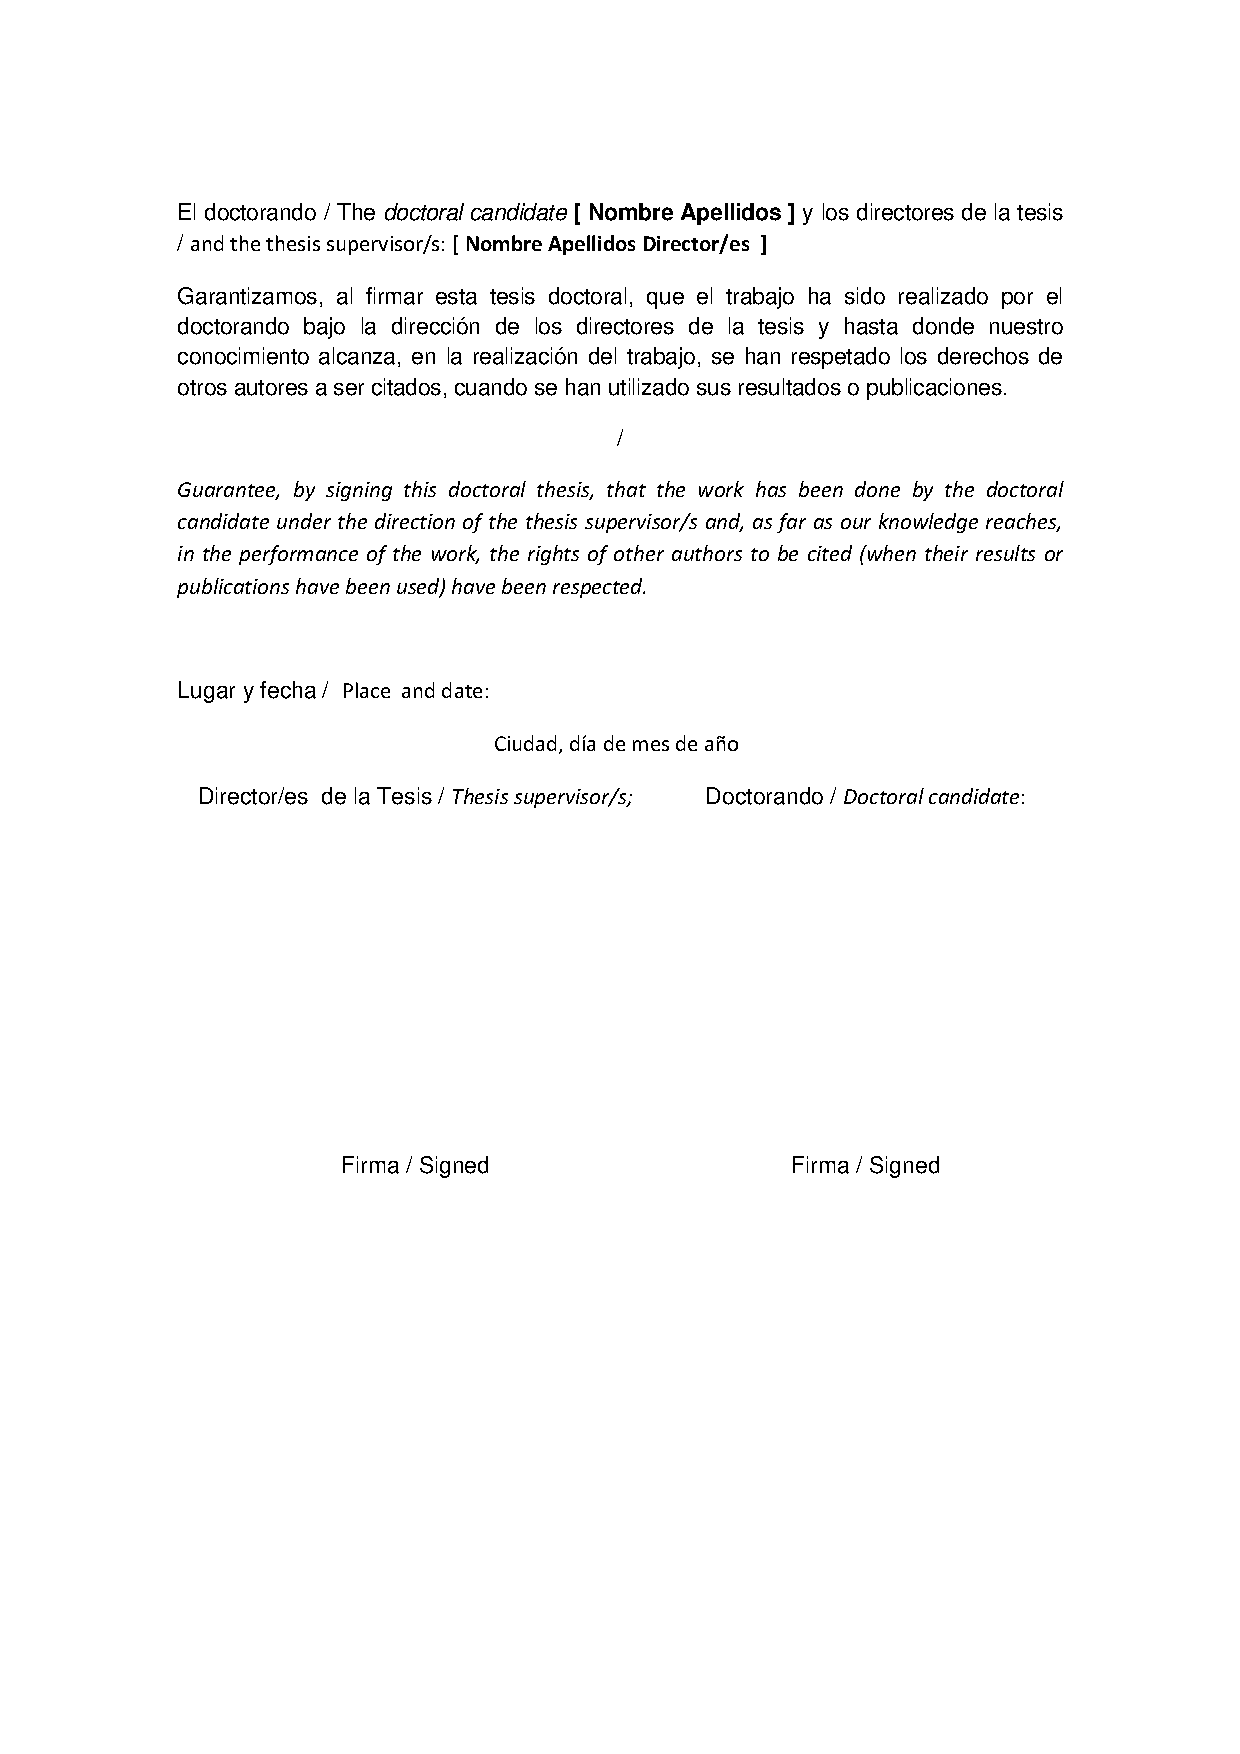
\includepdf[offset=15 0]{declaraciones/Compromiso_derechos_autor_tesis_firmado.pdf}
\newpage
\thispagestyle{empty}
\mbox{}
\newpage
{\large\bf Acrónimos}
\printacronyms[heading=none]
\newpage
\thispagestyle{empty}

% Numeración de páginas con números romanos previa a los capítulos.
\singlespacing
\pagenumbering{Roman}
\setcounter{page}{11}
\body

\chapter*{Resumen}\label{capitulo:Resumen}
\markboth{Resumen}{}

%\mtcaddchapter[Resumen] %Para añadirlo al indice y que no genere conflicto con el paquete minitoc

\section*{Introducción al problema}\label{seccion:IntroduccionProblema}

Introducción al problema abordado.

\section*{Desarrollo}\label{seccion:Desarrollo}

Bloques desarrollo de tesis: 

\begin{enumerate}[label=\Roman*]
	\item Bloque A.
	\item Bloque B. 
	\item Bloque C.
\end{enumerate}

Introducción a secciones tesis. 

\subsection*{Sección uno}\label{seccion:SeccionUno}

Iniciamos \dots 

\subsection*{Sección dos}\label{seccion:SeccionDos}

Tras finalizar la Sección~\ref{seccion:SeccionUno} \dots

\subsection*{Sección tres}\label{seccion:SeccionTres}

Como ya mencionamos en \dots 

\subsection*{Sección cuatro}\label{seccion:SeccionCuatro}

Por último \dots

\section*{Conclusiones y trabajos futuros}\label{seccion:ConclusionesResumen}

En conclusión \dots


\addcontentsline{toc}{chapter}{Resumen}
\clearpage
\chapter*{Abstract}\label{capitulo:Abstract}
\markboth{}{}
%\newpage
%\thispagestyle{empty}
%\mbox{}
%\newpage

%\mtcaddchapter[Resumen] %Para añadirlo al indice y que no genere conflicto con el paquete minitoc

%\begin{resumen}
%
%\mtcaddchapter[Resumen] %Para añadirlo al indice y que no genere conflicto con el paquete minitoc

\section*{Introducción al problema}\label{seccion:IntroduccionProblema}

Introducción al problema abordado.

\section*{Desarrollo}\label{seccion:Desarrollo}

Bloques desarrollo de tesis: 

\begin{enumerate}[label=\Roman*]
	\item Bloque A.
	\item Bloque B. 
	\item Bloque C.
\end{enumerate}

Introducción a secciones tesis. 

\subsection*{Sección uno}\label{seccion:SeccionUno}

Iniciamos \dots 

\subsection*{Sección dos}\label{seccion:SeccionDos}

Tras finalizar la Sección~\ref{seccion:SeccionUno} \dots

\subsection*{Sección tres}\label{seccion:SeccionTres}

Como ya mencionamos en \dots 

\subsection*{Sección cuatro}\label{seccion:SeccionCuatro}

Por último \dots

\section*{Conclusiones y trabajos futuros}\label{seccion:ConclusionesResumen}

En conclusión \dots


%\end{resumen}
    
%\newpage
%\thispagestyle{empty}
%\mbox{}
%\newpage

%\mtcaddchapter[Abstract]

Abstract written in English \dots
\addcontentsline{toc}{chapter}{Abstract}
\clearpage
\chapter{Introducción}\label{capitulo:Introduccion}

\epigraph{Cita.}{Autor}

\section{Introducción}\label{seccion:Introduccion}

\section{Objetivos}\label{seccion:Objetivos}

En esta tesis hemos de cumplir los siguientes objetivos específicos:

\begin{itemize}
	\item En nuestro \textbf{primer objetivo} \dots
	\item Un \textbf{segundo objetivo} \dots
    \item Un \textbf{tercer objetivo} \dots
\end{itemize}

\section{Estructura}\label{seccion:Estructura}

Esta tesis doctoral se divide en tres partes: Fundamentos, Propuesta y Observaciones finales, además de la presente introducción. 

La primera parte introduce al lector en los fundamentos de varias teorías y metodologías \dots En el capítulo~\ref{capitulo:CapituloUno} se \dots A continuación, en el capítulo~\ref{capitulo:CapituloDos}, se \dots

La segunda parte (Propuesta) desarrolla \dots Por un lado, el capítulo~\ref{capitulo:CapituloTres} describe \dots

Por último, la tercera parte (Observaciones finales), consta de un único capítulo (capítulo~\ref{capitulo:Conclusiones}) en el que \dots
\clearpage
\part{Fundamentos}
\clearpage
\chapter{Capítulo dos}\label{capitulo:CapituloDos}
\epigraph{Cita}{Autor}

\section{Sección uno}\label{seccion:SeccionUnoCapituloUno}

Las sociedades~\cite{citaEjemplo23} \dots
	
\section{Sección dos}\label{seccion:SeccionDosCapituloUno}

Una de \dots

\begin{itemize}
	\item \textbf{Uno}: Los \dots
	\item \textbf{Dos}: Los \dots
	\item \textbf{Tres}: Los \dots
	\item \textbf{Cuatro}: Los \dots
	\item \textbf{Cinco}: Los \dots
\end{itemize}

\section{Sección tres}\label{seccion:SeccionTresCapituloUno}

El acrónimo uno (\acsp{AO}, por sus siglas en inglés) \dots

\subsection{Subsección uno}\label{subsection:SubseccionUnoSeccionTresCapituloUno} 

\subsection{Subsección dos}\label{subseccion:SubseccionDosSeccionTresCapituloUno}

Las \dots

La Figura~\ref{figura:EjemploUno}
\begin{figure}[!ht]
	\centering
	\includesvg[width=7cm]{imagenes/logoUGR.svg}
	\caption{Figura de ejemplo}
	\label{figura:EjemploUno}
\end{figure}

\iffalse % Para guardar texto redactado como comentario para su posterior reutilización
\begin{itemize}
	\item \textbf{Ejemplo uno}:  
	\item \textbf{Ejemplo dos}: 
	\item \textbf{Ejemplo tres}: 
\end{itemize}
\fi

\subsubsection{Subsubsección uno}\label{subsubseccion:SubsubseccionUnoSubseccionUnoSeccionTresCapituloUno}

\subsubsection{Subsubsección dos}\label{subsubseccion:SubsubseccionDosSubseccionUnoSeccionTresCapituloUno}

\subsubsection{Subsubsección tres}\label{subsubseccion:SubsubseccionTresSubseccionUnoSeccionTresCapituloUno}

\subsection{Subsección tres}\label{subseccion:SubseccionTresSeccionTresCapituloUno} 

\subsubsection{Subsubsección uno}\label{subsubseccion:SubsubseccionUnoSubseccionTresSeccionTresCapituloUno}
\chapter{Capítulo tres}\label{capitulo:CapituloTres}
\epigraph{Cita.}{Autor}

\section{Sección uno}\label{seccion:SeccionUnoCapituloDos}

Como vimos en la Sección~\ref{seccion:SeccionUnoCapituloUno}, la tesis \dots

\section{Sección dos}\label{seccion:SeccionDosCapituloDos}
\clearpage
\part{Propuesta}
\clearpage
\chapter{Capítulo cuatro}\label{capitulo:CapituloCuatro}

\epigraph{Cita.}{Autor}

\section{Sección uno}\label{seccion:SeccionUnoCapituloTres}

En el Capítulo~\ref{capitulo:CapituloTres} expusimos \dots 

En la Table~\ref{tabla:EjemploUno} \dots

\begin{table}[H]
	\centering
	\footnotesize
	\begin{tabular}{|c||l||l|}
		\hline
		\textbf{Columna uno} & \textbf{Columna dos} & \textbf{Columna tres} \\ \hline \hline
		$A$ & I & 1\\ \hline
		$B$ & II & 2\\ \hline
		$C$ & III & 3\\ \hline
		$D$ & IV & 4\\ \hline
		$E$ & V & 5 \\ \hline
		\multirow{2}{*}{$F$} & \multirow{2}{*}{VI} & \multirow{2}{*}{\begin{tabular}[c]{@{}l@{}} $6, 7, 8, 9,$ \\  $10, 11, 12, 13$ \end{tabular}} \\ 
		& & \\ \hline
		\multirow{2}{*}{$G$} & \multirow{2}{*}{VII} & \multirow{2}{*}{\begin{tabular}[c]{@{}l@{}} $8, 9, 10, 11,$ \\ $10, 9, 8, 7$ \end{tabular}} \\
		& & \\
		\bottomrule
	\end{tabular}
	\caption{Tabla de ejemplo.}
	\label{tabla:EjemploUno}
\end{table}
\clearpage
\part{Observaciones finales}
\clearpage
\chapter{Conclusiones y trabajos futuros}\label{capitulo:Conclusiones}
\epigraph{Los hombres geniales empiezan grandes obras, los hombres trabajadores las terminan.}{Leonardo da Vinci}

\section{Conclusiones}\label{seccion:Conclusiones}

Las principales conclusiones de esta tesis son \dots 

\section{Publicaciones}\label{seccion:Publicaciones}

Por último, esta sección presenta las publicaciones científicas realizadas en el curso de esta tesis doctoral.

\textbf{Artículos publicados en revistas indexadas en el JCR-SCI (X):}

\begin{enumerate}
    \item Surname author I, Name author I, Surname author II, \& Name author II, O. (Year). \textbf{Paper Title}. Journal, Number, Pages. DOI: doi-number (JCR Year; impact: factor; Cat.: CATEGORY; Pos.: Possition; Q1). Relacionado con el Capítulo~\ref{capitulo:CapituloDos}. 
    \item Surname author I, Name author I, Surname author II, \& Name author II, O. (Year). \textbf{Paper Title}. Journal, Number, Pages. DOI: doi-number (JCR Year; impact: factor; Cat.: CATEGORY; Pos.: Possition; Q1). Relacionado con el Capítulo~\ref{capitulo:CapituloTres}. 
\end{enumerate}

\textbf{Artículos publicados en revistas no indexadas en el JCR-SCI (Y):}

\begin{enumerate}
    \item Surname author I, Name author I, Surname author II, \& Name author II, O. (Year). \textbf{Paper Title}. Journal, Number, Pages. DOI: doi-number (JCR Year; impact: factor; Cat.: CATEGORY; Pos.: Possition; Q1). Relacionado con el Capítulo~\ref{capitulo:CapituloCuatro}. 
\end{enumerate}

\textbf{Artículos publicados en congresos internacionales (Z):}

\begin{enumerate}
    \item Surname author I, Name author I, Surname author II, \& Name author II, O. (Year). \textbf{Paper Title}. Journal, Number, Pages. DOI: doi-number (JCR Year; impact: factor; Cat.: CATEGORY; Pos.: Possition; Q1). Relacionado con el Capítulo~\ref{capitulo:CapituloUno}.
   \item Surname author I, Name author I, Surname author II, \& Name author II, O. (Year). \textbf{Paper Title}. Journal, Number, Pages. DOI: doi-number (JCR Year; impact: factor; Cat.: CATEGORY; Pos.: Possition; Q1). Relacionado con el Capítulo~\ref{capitulo:CapituloTres}.
\end{enumerate}

\textbf{Artículos publicados en congresos nacionales (K):}

\begin{enumerate}
    \item Surname author I, Name author I, Surname author II, \& Name author II, O. (Year). \textbf{Paper Title}. Journal, Number, Pages. DOI: doi-number (JCR Year; impact: factor; Cat.: CATEGORY; Pos.: Possition; Q1). Relacionado con el Capítulo~\ref{capitulo:CapituloCuatro}.
\end{enumerate}

\section{Agradecimientos}\label{seccion:Agradecimientos}

Esta tesis doctoral ha sido apoyada por \dots
\clearpage

\addcontentsline{toc}{chapter}{Bibliografía}
\printbibliography

\end{document}

%%%%%%%%%%%%%%%%%%%%%%%%%%%%%
%% ACRÓNIMOS
%%%%%%%%%%%%%%%%%%%%%%%%%%%%%
% Acrónimos Inglés
\DeclareAcronym{AO}{
	short = AI ,
	short-plural = es,
	long = {Acronym One},
	long-plural = es ,
	pdfcomment = {Acronym One}
}
%%%%%%%%%%%%%%%%%%%%%%%%%%
%%% FIN ACRÓNIMOS
%%%%%%%%%%%%%%%%%%%%%%%%%%

\begin{document}

\title{\hrule\LARGE {\bf Título Tesis\vspace*{2mm}\hrule}\par
 \vspace*{6mm}
}

\author{\textbf{Nombre y Apellidos Doctorando}}

\normallinespacing

\maketitle

%\preface % Eliminado porque añade dos páginas blancas tras primera entrada del documento. 
\newpage
\thispagestyle{empty}
\mbox{}
\newpage
\narrowlinespacing

\vspace*{5cm}

\epigraph{Primera cita.}{Autor}

\normallinespacing
\newpage
\thispagestyle{empty}
\mbox{}
\newpage

\begin{acknowledgements}

Agradecimientos de la tesis. La parte más importante de la tesis.

\begin{center}
Mensaje centrado.
\end{center}

\end{acknowledgements}
\newpage
\thispagestyle{empty}
\mbox{}
\newpage
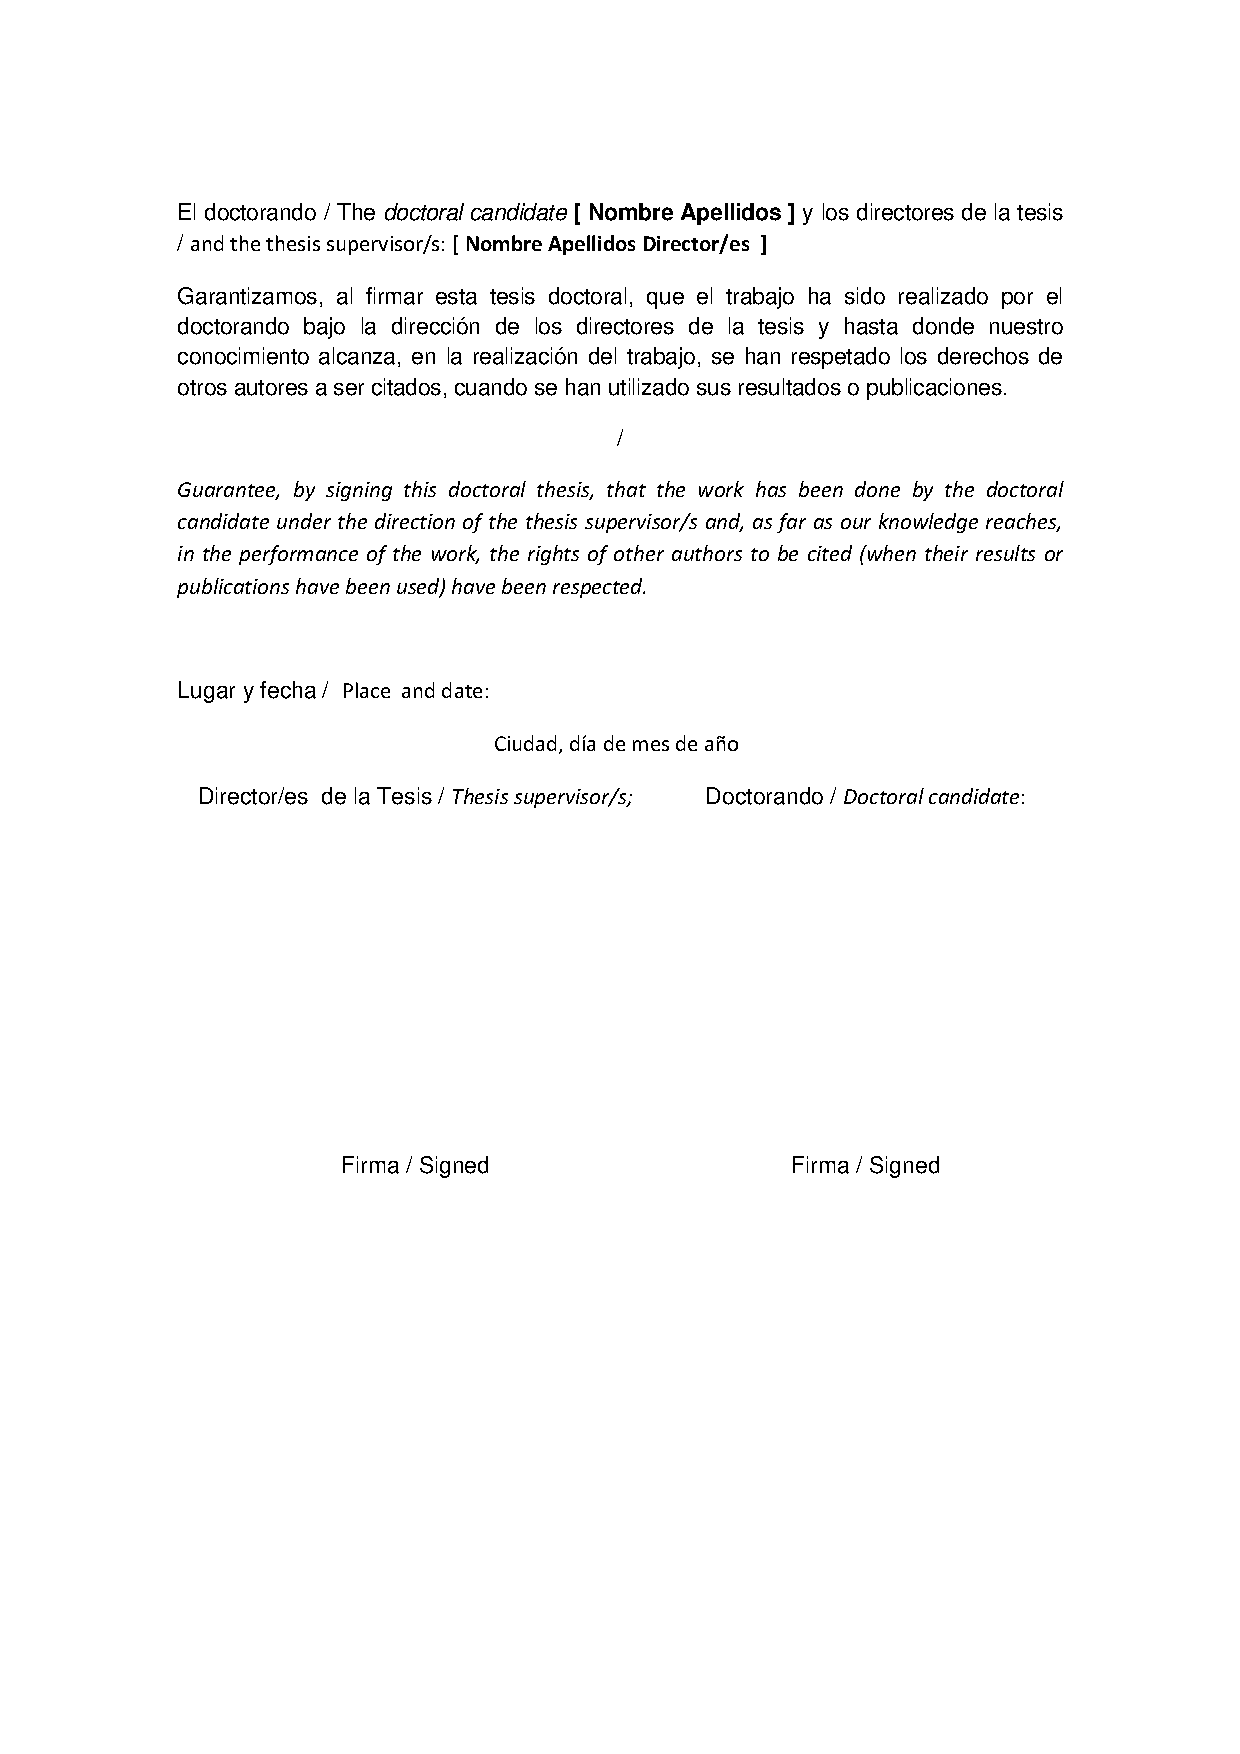
\includepdf[offset=15 0]{declaraciones/Compromiso_derechos_autor_tesis_firmado.pdf}
\newpage
\thispagestyle{empty}
\mbox{}
\newpage
{\large\bf Acrónimos}
\printacronyms[heading=none]
\newpage
\thispagestyle{empty}

% Numeración de páginas con números romanos previa a los capítulos.
\singlespacing
\pagenumbering{Roman}
\setcounter{page}{11}
\body

\chapter*{Resumen}\label{capitulo:Resumen}
\markboth{Resumen}{}

%\mtcaddchapter[Resumen] %Para añadirlo al indice y que no genere conflicto con el paquete minitoc

\section*{Introducción al problema}\label{seccion:IntroduccionProblema}

Introducción al problema abordado.

\section*{Desarrollo}\label{seccion:Desarrollo}

Bloques desarrollo de tesis: 

\begin{enumerate}[label=\Roman*]
	\item Bloque A.
	\item Bloque B. 
	\item Bloque C.
\end{enumerate}

Introducción a secciones tesis. 

\subsection*{Sección uno}\label{seccion:SeccionUno}

Iniciamos \dots 

\subsection*{Sección dos}\label{seccion:SeccionDos}

Tras finalizar la Sección~\ref{seccion:SeccionUno} \dots

\subsection*{Sección tres}\label{seccion:SeccionTres}

Como ya mencionamos en \dots 

\subsection*{Sección cuatro}\label{seccion:SeccionCuatro}

Por último \dots

\section*{Conclusiones y trabajos futuros}\label{seccion:ConclusionesResumen}

En conclusión \dots


\addcontentsline{toc}{chapter}{Resumen}
\clearpage
\chapter*{Abstract}\label{capitulo:Abstract}
\markboth{}{}
%\newpage
%\thispagestyle{empty}
%\mbox{}
%\newpage

%\mtcaddchapter[Resumen] %Para añadirlo al indice y que no genere conflicto con el paquete minitoc

%\begin{resumen}
%
%\mtcaddchapter[Resumen] %Para añadirlo al indice y que no genere conflicto con el paquete minitoc

\section*{Introducción al problema}\label{seccion:IntroduccionProblema}

Introducción al problema abordado.

\section*{Desarrollo}\label{seccion:Desarrollo}

Bloques desarrollo de tesis: 

\begin{enumerate}[label=\Roman*]
	\item Bloque A.
	\item Bloque B. 
	\item Bloque C.
\end{enumerate}

Introducción a secciones tesis. 

\subsection*{Sección uno}\label{seccion:SeccionUno}

Iniciamos \dots 

\subsection*{Sección dos}\label{seccion:SeccionDos}

Tras finalizar la Sección~\ref{seccion:SeccionUno} \dots

\subsection*{Sección tres}\label{seccion:SeccionTres}

Como ya mencionamos en \dots 

\subsection*{Sección cuatro}\label{seccion:SeccionCuatro}

Por último \dots

\section*{Conclusiones y trabajos futuros}\label{seccion:ConclusionesResumen}

En conclusión \dots


%\end{resumen}
    
%\newpage
%\thispagestyle{empty}
%\mbox{}
%\newpage

%\mtcaddchapter[Abstract]

Abstract written in English \dots
\addcontentsline{toc}{chapter}{Abstract}
\clearpage
\chapter{Introducción}\label{capitulo:Introduccion}

\epigraph{Cita.}{Autor}

\section{Introducción}\label{seccion:Introduccion}

\section{Objetivos}\label{seccion:Objetivos}

En esta tesis hemos de cumplir los siguientes objetivos específicos:

\begin{itemize}
	\item En nuestro \textbf{primer objetivo} \dots
	\item Un \textbf{segundo objetivo} \dots
    \item Un \textbf{tercer objetivo} \dots
\end{itemize}

\section{Estructura}\label{seccion:Estructura}

Esta tesis doctoral se divide en tres partes: Fundamentos, Propuesta y Observaciones finales, además de la presente introducción. 

La primera parte introduce al lector en los fundamentos de varias teorías y metodologías \dots En el capítulo~\ref{capitulo:CapituloUno} se \dots A continuación, en el capítulo~\ref{capitulo:CapituloDos}, se \dots

La segunda parte (Propuesta) desarrolla \dots Por un lado, el capítulo~\ref{capitulo:CapituloTres} describe \dots

Por último, la tercera parte (Observaciones finales), consta de un único capítulo (capítulo~\ref{capitulo:Conclusiones}) en el que \dots
\clearpage
\part{Fundamentos}
\clearpage
\chapter{Capítulo dos}\label{capitulo:CapituloDos}
\epigraph{Cita}{Autor}

\section{Sección uno}\label{seccion:SeccionUnoCapituloUno}

Las sociedades~\cite{citaEjemplo23} \dots
	
\section{Sección dos}\label{seccion:SeccionDosCapituloUno}

Una de \dots

\begin{itemize}
	\item \textbf{Uno}: Los \dots
	\item \textbf{Dos}: Los \dots
	\item \textbf{Tres}: Los \dots
	\item \textbf{Cuatro}: Los \dots
	\item \textbf{Cinco}: Los \dots
\end{itemize}

\section{Sección tres}\label{seccion:SeccionTresCapituloUno}

El acrónimo uno (\acsp{AO}, por sus siglas en inglés) \dots

\subsection{Subsección uno}\label{subsection:SubseccionUnoSeccionTresCapituloUno} 

\subsection{Subsección dos}\label{subseccion:SubseccionDosSeccionTresCapituloUno}

Las \dots

La Figura~\ref{figura:EjemploUno}
\begin{figure}[!ht]
	\centering
	\includesvg[width=7cm]{imagenes/logoUGR.svg}
	\caption{Figura de ejemplo}
	\label{figura:EjemploUno}
\end{figure}

\iffalse % Para guardar texto redactado como comentario para su posterior reutilización
\begin{itemize}
	\item \textbf{Ejemplo uno}:  
	\item \textbf{Ejemplo dos}: 
	\item \textbf{Ejemplo tres}: 
\end{itemize}
\fi

\subsubsection{Subsubsección uno}\label{subsubseccion:SubsubseccionUnoSubseccionUnoSeccionTresCapituloUno}

\subsubsection{Subsubsección dos}\label{subsubseccion:SubsubseccionDosSubseccionUnoSeccionTresCapituloUno}

\subsubsection{Subsubsección tres}\label{subsubseccion:SubsubseccionTresSubseccionUnoSeccionTresCapituloUno}

\subsection{Subsección tres}\label{subseccion:SubseccionTresSeccionTresCapituloUno} 

\subsubsection{Subsubsección uno}\label{subsubseccion:SubsubseccionUnoSubseccionTresSeccionTresCapituloUno}
\chapter{Capítulo tres}\label{capitulo:CapituloTres}
\epigraph{Cita.}{Autor}

\section{Sección uno}\label{seccion:SeccionUnoCapituloDos}

Como vimos en la Sección~\ref{seccion:SeccionUnoCapituloUno}, la tesis \dots

\section{Sección dos}\label{seccion:SeccionDosCapituloDos}
\clearpage
\part{Propuesta}
\clearpage
\chapter{Capítulo cuatro}\label{capitulo:CapituloCuatro}

\epigraph{Cita.}{Autor}

\section{Sección uno}\label{seccion:SeccionUnoCapituloTres}

En el Capítulo~\ref{capitulo:CapituloTres} expusimos \dots 

En la Table~\ref{tabla:EjemploUno} \dots

\begin{table}[H]
	\centering
	\footnotesize
	\begin{tabular}{|c||l||l|}
		\hline
		\textbf{Columna uno} & \textbf{Columna dos} & \textbf{Columna tres} \\ \hline \hline
		$A$ & I & 1\\ \hline
		$B$ & II & 2\\ \hline
		$C$ & III & 3\\ \hline
		$D$ & IV & 4\\ \hline
		$E$ & V & 5 \\ \hline
		\multirow{2}{*}{$F$} & \multirow{2}{*}{VI} & \multirow{2}{*}{\begin{tabular}[c]{@{}l@{}} $6, 7, 8, 9,$ \\  $10, 11, 12, 13$ \end{tabular}} \\ 
		& & \\ \hline
		\multirow{2}{*}{$G$} & \multirow{2}{*}{VII} & \multirow{2}{*}{\begin{tabular}[c]{@{}l@{}} $8, 9, 10, 11,$ \\ $10, 9, 8, 7$ \end{tabular}} \\
		& & \\
		\bottomrule
	\end{tabular}
	\caption{Tabla de ejemplo.}
	\label{tabla:EjemploUno}
\end{table}
\clearpage
\part{Observaciones finales}
\clearpage
\chapter{Conclusiones y trabajos futuros}\label{capitulo:Conclusiones}
\epigraph{Los hombres geniales empiezan grandes obras, los hombres trabajadores las terminan.}{Leonardo da Vinci}

\section{Conclusiones}\label{seccion:Conclusiones}

Las principales conclusiones de esta tesis son \dots 

\section{Publicaciones}\label{seccion:Publicaciones}

Por último, esta sección presenta las publicaciones científicas realizadas en el curso de esta tesis doctoral.

\textbf{Artículos publicados en revistas indexadas en el JCR-SCI (X):}

\begin{enumerate}
    \item Surname author I, Name author I, Surname author II, \& Name author II, O. (Year). \textbf{Paper Title}. Journal, Number, Pages. DOI: doi-number (JCR Year; impact: factor; Cat.: CATEGORY; Pos.: Possition; Q1). Relacionado con el Capítulo~\ref{capitulo:CapituloDos}. 
    \item Surname author I, Name author I, Surname author II, \& Name author II, O. (Year). \textbf{Paper Title}. Journal, Number, Pages. DOI: doi-number (JCR Year; impact: factor; Cat.: CATEGORY; Pos.: Possition; Q1). Relacionado con el Capítulo~\ref{capitulo:CapituloTres}. 
\end{enumerate}

\textbf{Artículos publicados en revistas no indexadas en el JCR-SCI (Y):}

\begin{enumerate}
    \item Surname author I, Name author I, Surname author II, \& Name author II, O. (Year). \textbf{Paper Title}. Journal, Number, Pages. DOI: doi-number (JCR Year; impact: factor; Cat.: CATEGORY; Pos.: Possition; Q1). Relacionado con el Capítulo~\ref{capitulo:CapituloCuatro}. 
\end{enumerate}

\textbf{Artículos publicados en congresos internacionales (Z):}

\begin{enumerate}
    \item Surname author I, Name author I, Surname author II, \& Name author II, O. (Year). \textbf{Paper Title}. Journal, Number, Pages. DOI: doi-number (JCR Year; impact: factor; Cat.: CATEGORY; Pos.: Possition; Q1). Relacionado con el Capítulo~\ref{capitulo:CapituloUno}.
   \item Surname author I, Name author I, Surname author II, \& Name author II, O. (Year). \textbf{Paper Title}. Journal, Number, Pages. DOI: doi-number (JCR Year; impact: factor; Cat.: CATEGORY; Pos.: Possition; Q1). Relacionado con el Capítulo~\ref{capitulo:CapituloTres}.
\end{enumerate}

\textbf{Artículos publicados en congresos nacionales (K):}

\begin{enumerate}
    \item Surname author I, Name author I, Surname author II, \& Name author II, O. (Year). \textbf{Paper Title}. Journal, Number, Pages. DOI: doi-number (JCR Year; impact: factor; Cat.: CATEGORY; Pos.: Possition; Q1). Relacionado con el Capítulo~\ref{capitulo:CapituloCuatro}.
\end{enumerate}

\section{Agradecimientos}\label{seccion:Agradecimientos}

Esta tesis doctoral ha sido apoyada por \dots
\clearpage

\addcontentsline{toc}{chapter}{Bibliografía}
\printbibliography

\end{document}